\subsubsection{Design}
\paragraph{Purpose}
The Medical Services Crew is responsible for managing and coordinating medical resources during emergency situations. This includes assessing hospital capacities, allocating resources, deploying paramedics, and ensuring timely medical response to incidents.

\paragraph{Changes}
Initially, the tasks of the Medical Services Crew were planned in a different order and with a distinct execution flow. A comparison of the initial and updated workflows is presented in \textbf{Figure} \ref{fig:exc_flow_ms_comparison}. In the updated process, the Recieve Report task was removed, since it was not necessary for the crew's operations. Additionally, the Rank Hospitals and Allocate Hospital Resources were each split into 2 separate tasks: Fetch Hospital Information and Rank Hospitals, and Plan Hospital Response and Allocate Hospital Resources, respectively. This restructuring was done to improve the efficiency and clarity of the crews' operations, since the tasks' results were poor when one agent had to perform too many steps at a time. We observed that the agents especially struggled when combining in a single task the use of a tool and the inference of logical results from said tool's output.

\begin{figure}[H]
    \centering
    \begin{subfigure}[b]{0.28\textwidth}
        \centering
        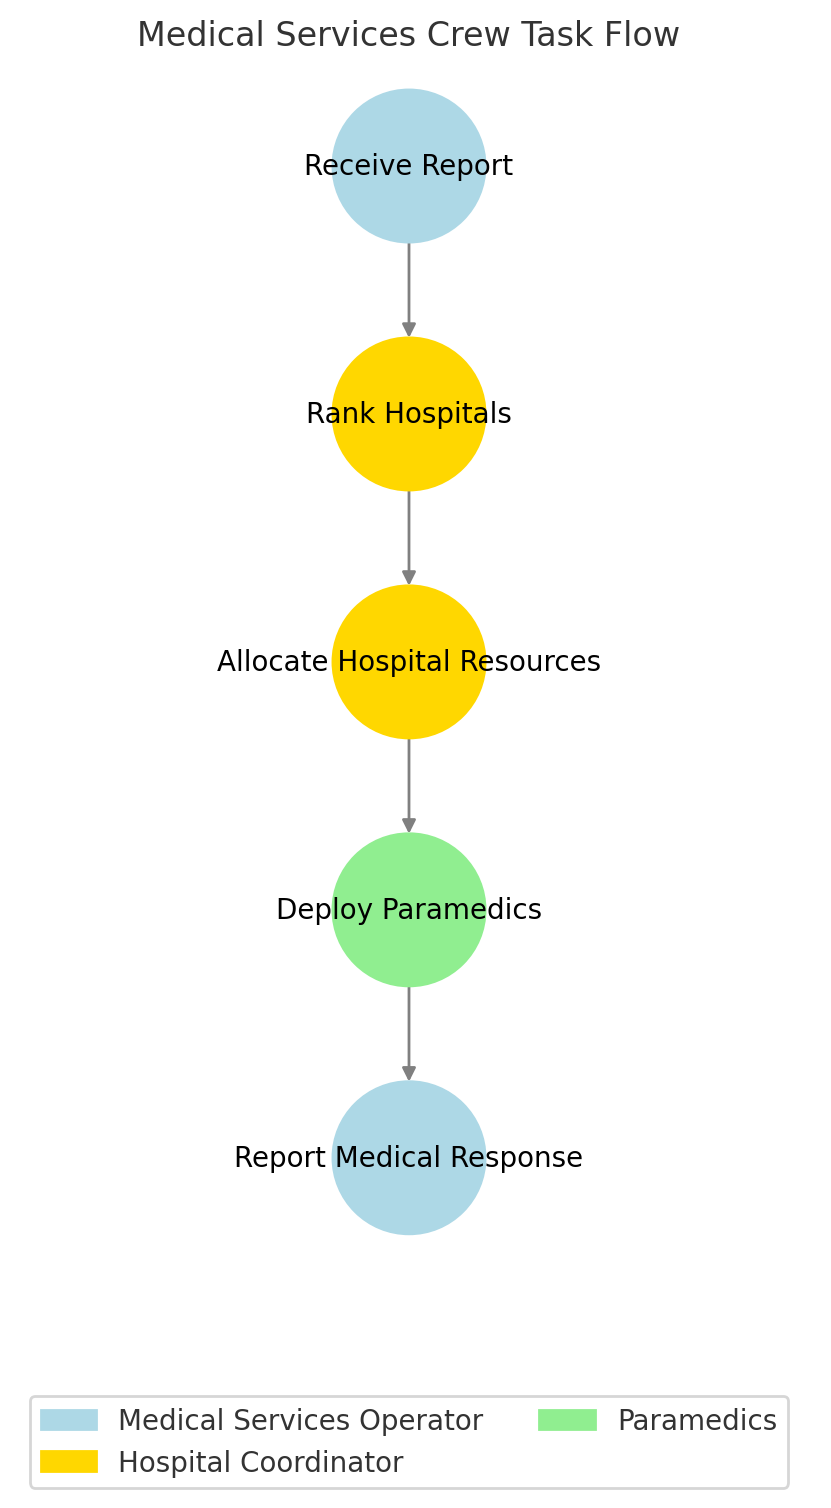
\includegraphics[width=\textwidth]{figures/Medical_Services_Crew_Flow.png}
        \caption{Initial process}
        \label{fig:initial_process}
    \end{subfigure}
    \hfill
    \begin{subfigure}[b]{0.7\textwidth}
        \centering
        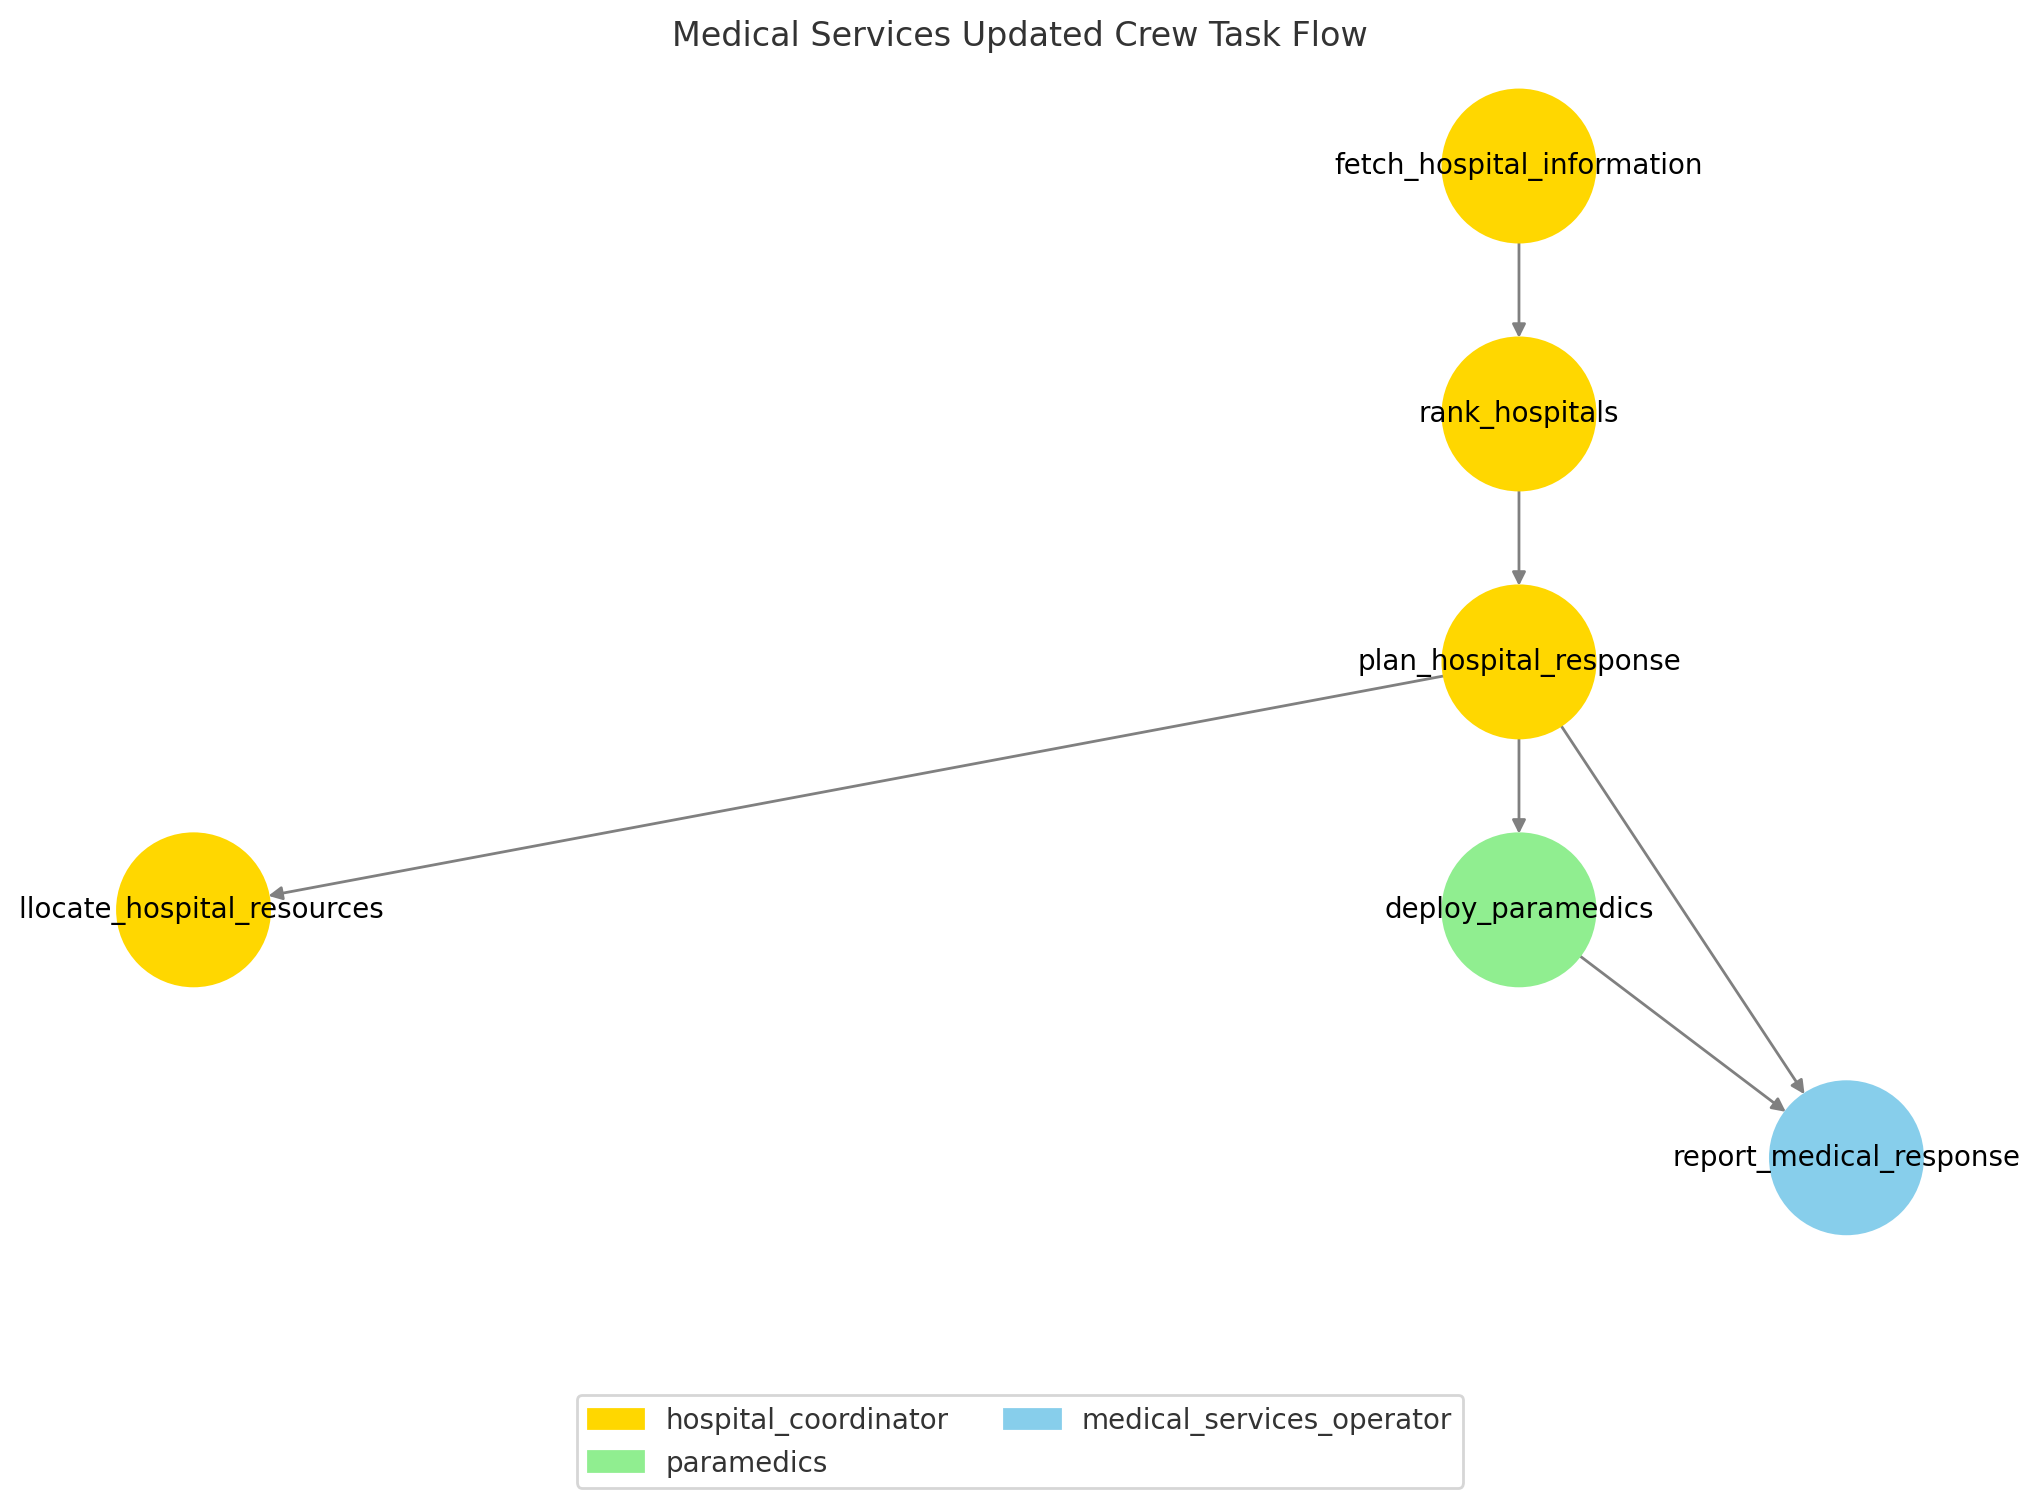
\includegraphics[width=\textwidth]{figures/Medical_Services_Crew_Flow_updated.png}
        \caption{Updated process}
        \label{fig:updated_process}
    \end{subfigure}
    \caption{Comparison of the Medical Services Crew's execution flow. (a) shows the initial process, while (b) illustrates the updated process with task restructuring for improved efficiency.}
    \label{fig:exc_flow_ms_comparison}
\end{figure}

\paragraph{Structure and Components}
The Medical Services Crew leverages the \texttt{CrewBase} framework to orchestrate its agents and tasks, ensuring cohesive and efficient operations. The key components of the design are:

\begin{itemize}
    \item \textbf{Agents:}
    \begin{itemize}
        \item \texttt{medical\_services\_operator}: Facilitates communication and coordination within the Medical Services crew and with other crews, ensuring efficient information flow and timely updates during emergencies.
        \item \texttt{hospital\_coordinator}: Manages all hospitals, decides each of their responses based on proximity to emergencies, and allocates resources effectively to ensure optimal response during crises.
        \item \texttt{paramedics}: Plans the deployment of paramedics to the emergency site, including the number of paramedics, ambulances, estimated times of arrival, and any special equipment needed to handle the situation effectively.
    \end{itemize}
    \item \textbf{Tasks:}
    \begin{itemize}
        \item \texttt{fetch\_hospital\_information}: Uses the Hospital Reader Tool to fetch the information of all hospitals from the database and returns the hospital information in a structured output.
        \item \texttt{rank\_hospitals}: Receives input containing the Medical Assessment and the hospital information from the previous task, calculates the distance to the emergency location using the Route Distance Tool, and returns the list of hospital information with distances to the emergency.
        \item \texttt{plan\_hospital\_response}: Reads the ranked list of hospitals and the Medical Assessment, assesses available resources at the given hospitals, and creates an allocation plan that details how resources will be utilized to address the emergency.
        \item \texttt{allocate\_hospital\_resources}: Reads the Hospital Resource Allocation plan, uses the Hospital Updater Tool to update the database for all of the hospital resources used in the plan, and confirms that the hospital resources have been successfully allocated.
        \item \texttt{deploy\_paramedics}: Reads the Hospital Resource Allocation plan and the Medical Assessment, calculates the total number of paramedics to be deployed and ambulances to be dispatched, determines the estimated times of arrival, and identifies any special equipment required.
        \item \texttt{report\_medical\_response}: Reads the Hospital Resource Allocation plan, the Paramedic Deployment plan, and the Medical Assessment, compiles a comprehensive summary of the medical response plan, and provides a detailed report for future reference and continuous improvement.
    \end{itemize}
    \item \textbf{Crew:}
    The crew is constructed using the \texttt{Crew} class, which integrates the agents and tasks into a seamless workflow. This design ensures effective progression from hospital information retrieval and resource allocation to paramedic deployment and medical response reporting.
\end{itemize}
The modular design of the Medical Services Crew enables it to adapt to a wide range of emergency scenarios, ensuring efficient and timely medical response to incidents.

